\documentclass[border=3pt]{standalone}
% Preâmbulo compartilhado pelos diagramas TikZ da aula 8 de IHR (Métodos de Pesquisa)
\usepackage[T1]{fontenc}
\usepackage[utf8]{inputenc}
\usepackage{lmodern}
\usepackage{amsmath}
\usepackage{xcolor}
\usepackage{tikz}
\usetikzlibrary{arrows.meta,angles,quotes,decorations.pathmorphing,decorations.pathreplacing,calc,
                positioning,shapes.geometric,shapes.misc,backgrounds,fit,
                math}

% Paleta (mesma dos SVGs originais)
% Paleta da disciplina de IHR: acento azul (#1A6FB5), cor de destaque do tema.
% (o nome "dblue" é mantido para não alterar todos os diagramas)
\definecolor{dblue}{HTML}{1A6FB5}
\definecolor{dorange}{HTML}{B3541E}
\definecolor{dgreen}{HTML}{4A7C59}
\definecolor{dred}{HTML}{9C4B4B}
\definecolor{dcream}{HTML}{F4F1EA}
\definecolor{dshade}{HTML}{DDD7C9}

% Função gaussiana (não normalizada por padrão de escala visual)
\pgfmathdeclarefunction{gauss}{3}{%
  \pgfmathparse{1/(#3*sqrt(2*pi))*exp(-((#1-#2)^2)/(2*#3^2))}%
}

% Estilos comuns (prefixo d... para não colidir com chaves internas do pgf)
\tikzset{
  >={Stealth[length=2mm]},
  dguide/.style={gray!55, dashed, line width=0.4pt},
  daxis/.style={gray!60, line width=0.7pt, ->},
  dbody/.style={fill=black!3, draw=black!80, line width=1pt},
  dacc/.style={draw=dblue, line width=1pt},
  dlbl/.style={black!55, font=\small},
  dsub/.style={black!45, font=\footnotesize},
  dstate/.style={circle, draw=black!80, fill=dcream, line width=1pt,
                 minimum size=17mm, font=\large, inner sep=1pt},
  dobs/.style={circle, draw=black!80, fill=dshade, line width=1pt,
               minimum size=14mm, font=\large, inner sep=1pt},
  dbox/.style={rounded corners=2pt, draw=black!80, fill=dcream, line width=1pt,
               align=center, inner sep=6pt},
  dop/.style={circle, draw=black!80, fill=white, line width=1pt,
              minimum size=6mm, inner sep=0pt, font=\small},
  dtrans/.style={->, dblue, line width=1pt},
  dmeas/.style={->, dorange, line width=1pt},
  dcurve/.style={line width=1pt, dblue},
  dcurveb/.style={line width=1.4pt, dorange},
}

\begin{document}
\hyphenpenalty=10000 \exhyphenpenalty=10000 \tolerance=9999 \emergencystretch=3em
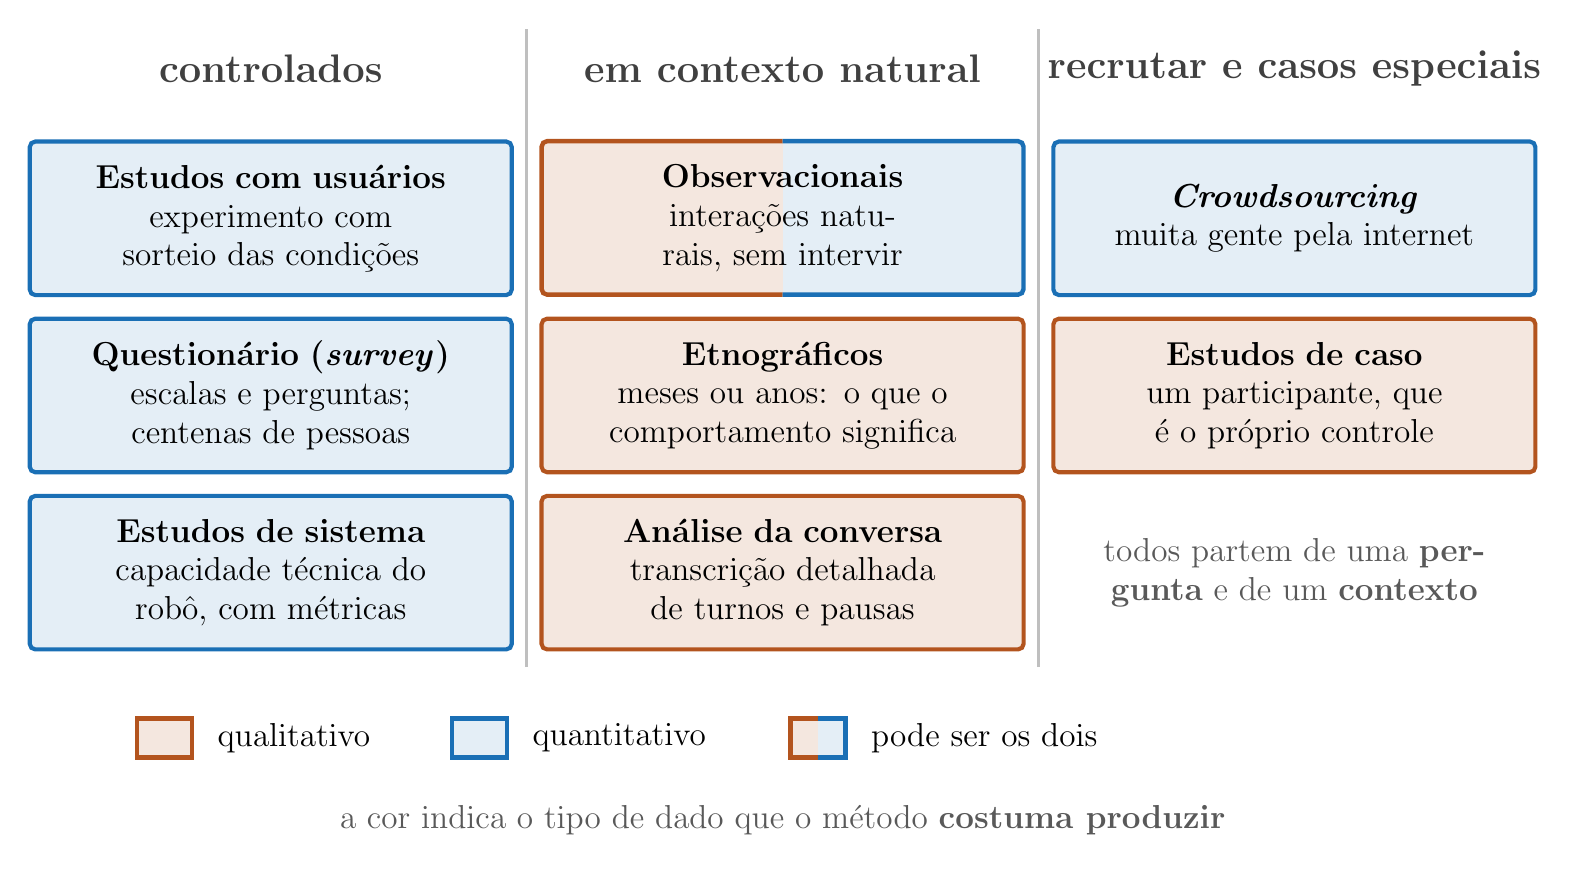
\begin{tikzpicture}[x=1cm,y=1cm]
  \tikzset{c/.style={dbox, text width=5.7cm, minimum height=1.95cm, font=\large, line width=1.5pt, align=center}}
  \draw[black!25, line width=1.2pt] (6.35,1.5) -- (6.35,9.6); \draw[black!25, line width=1.2pt] (12.85,1.5) -- (12.85,9.6);
  \node[font=\Large\bfseries, black!75] at (3.1,9.1) {controlados};
  \node[font=\Large\bfseries, black!75] at (9.6,9.1) {em contexto natural};
  \node[font=\Large\bfseries, black!75] at (16.1,9.1) {recrutar e casos especiais};
  \node[c, draw=dblue, fill=dblue!12] at (3.1,7.2) {\textbf{Estudos com usuários}\\ experimento com sorteio das condições};
  \node[c, draw=dblue, fill=dblue!12] at (3.1,4.95) {\textbf{Questionário (\emph{survey})}\\ escalas e perguntas; centenas de pessoas};
  \node[c, draw=dblue, fill=dblue!12] at (3.1,2.7) {\textbf{Estudos de sistema}\\ capacidade técnica do robô, com métricas};
  \begin{scope}\clip[rounded corners=2pt] (6.54,6.23) rectangle (12.66,8.18);
    \fill[dorange!14] (6.54,6.23) rectangle (9.60,8.18);
    \fill[dblue!12] (9.60,6.23) rectangle (12.66,8.18);
  \end{scope}
  \draw[dorange, line width=1.6pt, rounded corners=2pt] (9.60,8.18) -- (6.54,8.18) -- (6.54,6.23) -- (9.60,6.23);
  \draw[dblue, line width=1.6pt, rounded corners=2pt] (9.60,8.18) -- (12.66,8.18) -- (12.66,6.23) -- (9.60,6.23);
  \node[c, draw=none, fill=none] at (9.6,7.2) {\textbf{Observacionais}\\ interações naturais, sem intervir};
  \node[c, draw=dorange, fill=dorange!14] at (9.6,4.95) {\textbf{Etnográficos}\\ meses ou anos: o que o comportamento significa};
  \node[c, draw=dorange, fill=dorange!14] at (9.6,2.7) {\textbf{Análise da conversa}\\ transcrição detalhada de turnos e pausas};
  \node[c, draw=dblue, fill=dblue!12] at (16.1,7.2) {\textbf{\emph{Crowdsourcing}}\\ muita gente pela internet};
  \node[c, draw=dorange, fill=dorange!14] at (16.1,4.95) {\textbf{Estudos de caso}\\ um participante, que é o próprio controle};
  \node[font=\large, black!65, text width=5.7cm, align=center] at (16.1,2.7) {todos partem de uma \textbf{pergunta} e de um \textbf{contexto}};
  \draw[dorange, fill=dorange!14, line width=1.6pt] (1.4,0.35) rectangle ++(0.7,0.5);
  \node[font=\large, anchor=west] at (2.3,0.6) {qualitativo};
  \draw[dblue, fill=dblue!12, line width=1.6pt] (5.4,0.35) rectangle ++(0.7,0.5);
  \node[font=\large, anchor=west] at (6.3,0.6) {quantitativo};
  \fill[dorange!14] (9.7,0.35) rectangle ++(0.35,0.5); \fill[dblue!12] (10.05,0.35) rectangle ++(0.35,0.5);
  \draw[dorange, line width=1.6pt] (10.05,0.35) -- (9.7,0.35) -- (9.7,0.85) -- (10.05,0.85);
  \draw[dblue, line width=1.6pt] (10.05,0.35) -- (10.4,0.35) -- (10.4,0.85) -- (10.05,0.85);
  \node[font=\large, anchor=west] at (10.6,0.6) {pode ser os dois};
  \node[font=\large, black!65] at (9.6,-0.45) {a cor indica o tipo de dado que o método \textbf{costuma produzir}};
\end{tikzpicture}
\end{document}
